\chapter{Experiment setup}
\indent
    Experiment setup is listed in this chapter including 5 parts, 
    that is, initialization method, activation functions, optimizers, loss function, and the data structure of linear layer.

\section{Initialization method}
\indent
    \textbf{He normal initialization} is used in this experiment (See Listing \ref{he}). \\
    This initialization method performs well empirically when neural networks include \code{ReLU} activation function by many researchers.
    \begin{lstlisting}[language=Python, caption={He normal initialization code.}, label={he}]
    dim_in = layers[i]
    dim_out = layers[i + 1]
    a = np.sqrt(6. / (dim_in + dim_out))
    std = np.sqrt(2. / ((1 + a ** 2) * dim_in))
    
    W = np.random.normal(loc=0., scale=std, size=[dim_out, dim_in])
    b = np.random.normal(loc=0., scale=std, size=[1, dim_out])\end{lstlisting}

\section{Activation functions}
\indent
    There are many activation functions, e.g., \code{LeakyReLU}, \code{ReLU}, \code{Sigmoid}, and etc. 
    In this experiment, 3 activation functions, \code{LeakyReLU}, \code{ReLU} and \code{Sigmoid} 
    (See Figures \ref{leaky-relu}, \ref{relu}, and \ref{sigmoid}), are implemented.

    \begin{figure}[H]
		\centering
		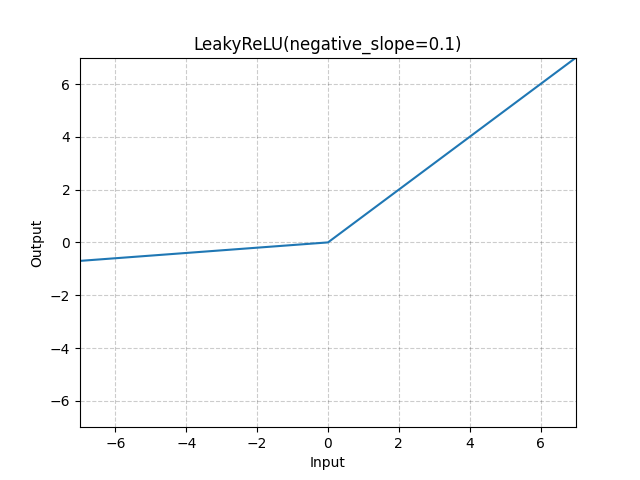
\includegraphics[scale=0.5]{img/leaky-relu.png}
		\caption{Illustration of LeakyReLU activation function.}
		\label{leaky-relu}
	\end{figure}
    \begin{figure}[H]
		\centering
		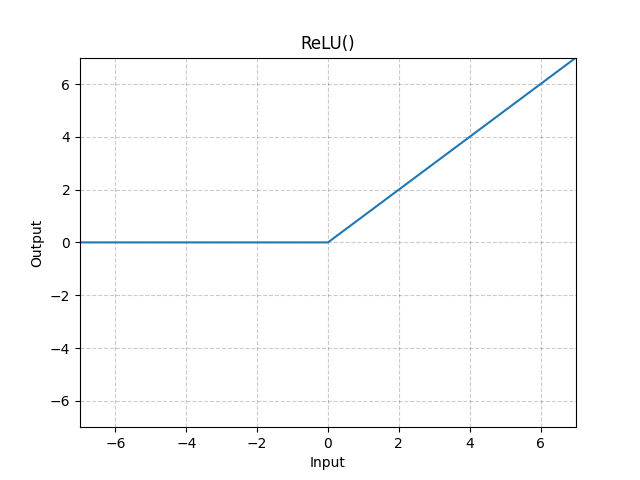
\includegraphics[scale=0.5]{img/relu.png}
		\caption{Illustration of ReLU activation function.}
		\label{relu}
	\end{figure}
    \begin{figure}[H]
		\centering
		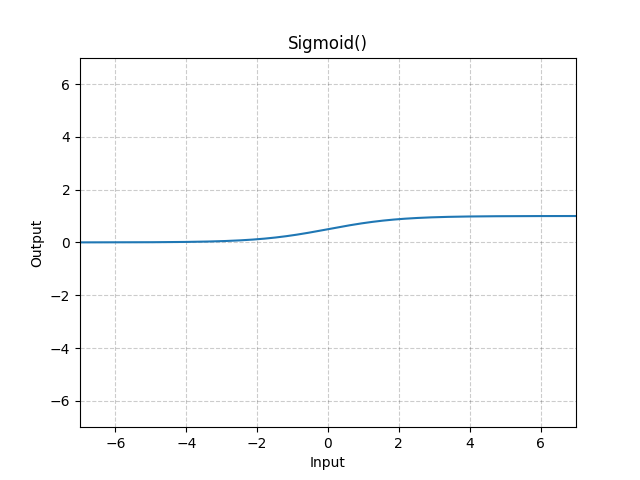
\includegraphics[scale=0.5]{img/sigmoid.png}
		\caption{Illustration of Sigmoid activation function.}
		\label{sigmoid}
	\end{figure}

\section{Optimizers}
\indent
    There are many optimizers, e.g., \code{SGD}, \code{Momentum}, \code{AdaGrad}, \code{Adam}, and etc.
    In this experiment, 2 optimizers, \code{SGD} (vanilla gradient descent in this case) and \code{Adam} (See Figure \ref{adam}) optimizers, are implemented. \\
    \code{Adam} optimizer is mostly used, and it has the great parts of \code{Momentum} and \code{AdaGrad}.

    \begin{figure}[H]
		\centering
		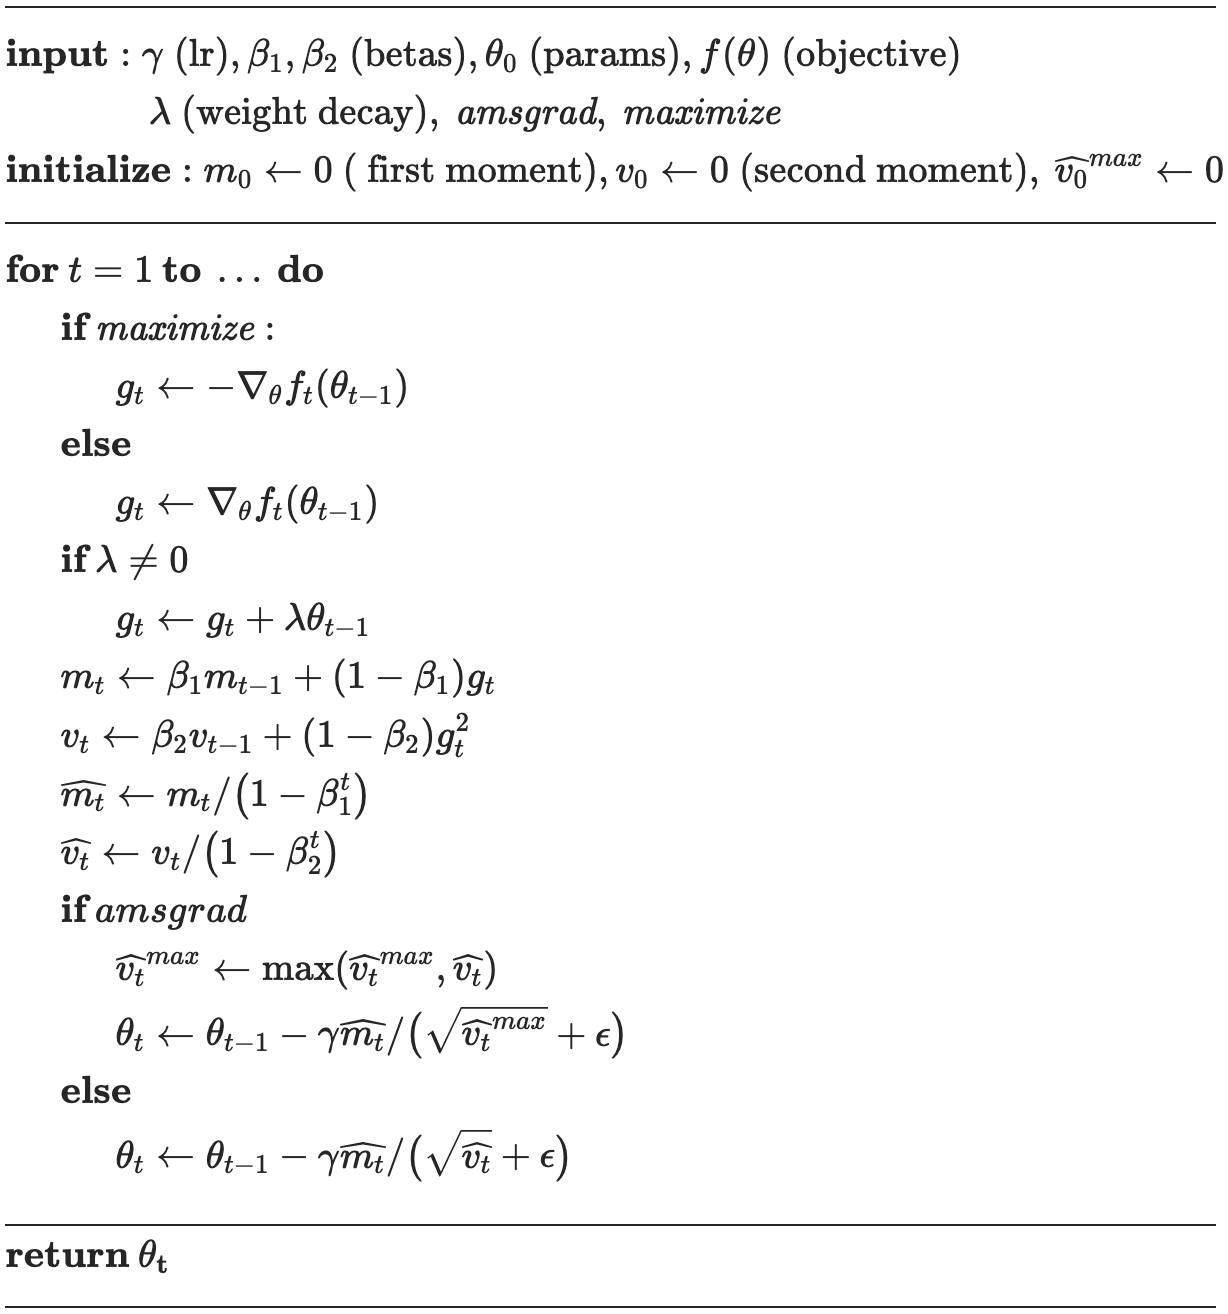
\includegraphics[scale=0.5]{img/adam.png}
		\caption{Pseudo code of Adam optimizer.}
		\label{adam}
	\end{figure}

\section{Loss function}
\indent
    \textbf{Cross entropy} (See Equation \ref{cross-entropy}) is used in this experiment, and it is also mostly used for classification tasks.
    \begin{equation}
        L(y, \hat{y}) = -[y\log\hat{y} + (1 - y)\log(1 - \hat{y})]
    \label{cross-entropy}
    \end{equation}
    where $y$ are ground truth labels and $\hat{y}$ are predicted labels.

\section{Data structure of linear layer}
\indent
    Data structure of linear layer is implemented using a class with only two member variables.
    It is well-defined, since \code{W} (weight matrix) and \code{b} (bias vector) are almost used at the same situations.
    \begin{lstlisting}[language=Python, caption={Date structure code of linear layer.}, label={linear-layer}]
    class Linear(object):      
        def __init__(self, W: np.ndarray, b: np.ndarray) -> None:
            self._W = W
            self._b = b
            
        @property
        def W(self) -> np.ndarray:
            return self._W
        
        @property
        def b(self) -> np.ndarray:
            return self._b
        
        @W.setter
        def W(self, W: np.ndarray) -> None:
            self._W = W
            
        @b.setter
        def b(self, b: np.ndarray) -> None:
            self._b = b
            
        def __str__(self) -> str:
            return f'<Linear W: {self._W.shape} b: {self._b.shape}>'\end{lstlisting}
